As with the original Prophet 600 firmware, there are two modes of operation, a \presetmode and a \livemode. You can change between the two by pressing the \preset button, see section \ref{datapad}. 

\textbf{Live mode vs. preset mode}

The idea of the \livemode (LED of preset button is off) is that the patch that is playing corresponds exactly to the parameters as currently set by all dials, switches and additional patch parameters. The synth produces the sound as set and seen. In \presetmode (LED of preset button is on), in contrast, the parameter values as stored in the patch memory are applied. The synth produces the sound of the preset. Still, once you change a dial or a switch on the panel or an additional parameter , this change will take effect also in \presetmode. In this case a "mixed state" applies, partly patch (untouched controls) and partly panel controls (touched controls). You can then store the current sound in the same patch or a different patch (See section \ref{loadstorepatches}). The patch will be stored as heard. 

Note that you also load a MIDI SysEx patch into the active patch parameters in \presetmode, see section \ref{patchmgmt}.

\textbf{Preset patch vs. preset panel mode}

In \presetmode the default setup is \presetpatch in which the \termnumberpad is used to select and load presets. However, in \presetmode you can also decide to switch to \presetpanel in which the \termnumberpad selects additional patch parameters similar to \livemode and the display shows the value of the last touched panel control. To activate this mode from \presetpatch, press \totape, after which the LED is on. To leave the \presetpanel, press \totape again. 

\textbf{Pick-me-up mode in preset panel mode}

The fact that the controls in \presetmode do not automatically correspond to the current active parameter values has two disadvantages. Firstly, once a control is touched it is immediately applied, irrespectively of where it is currently pointing and how far away that value is from the one used in the patch you are hearing. This may lead to unwanted, disruptive sound changes. Secondly, it may be difficult or cumbersome to retrieve an original patch value once it is changed using a control. Therefore, as of version \version the upgraded Prophet 600 supports a \textit{pick-me-up} control logic for dials in \presetpanel. It works as follows:

If you touch and change a dial the display indicates if the current active value is below the current dial position (arrow on the left) or above it (arrows on the right). As long a these arrows are shown the value of the dial will not be applied, it is not "picked up". Once you touch the current active value closely enough the display switches to showing the numerical value instead, indicating that the dial is "picked up". From that moment on all movements of the dial are always applied. If you move a dial fast enough you can hover over the pick-up point. The logic is shown below.

\scalebox{0.4}{
  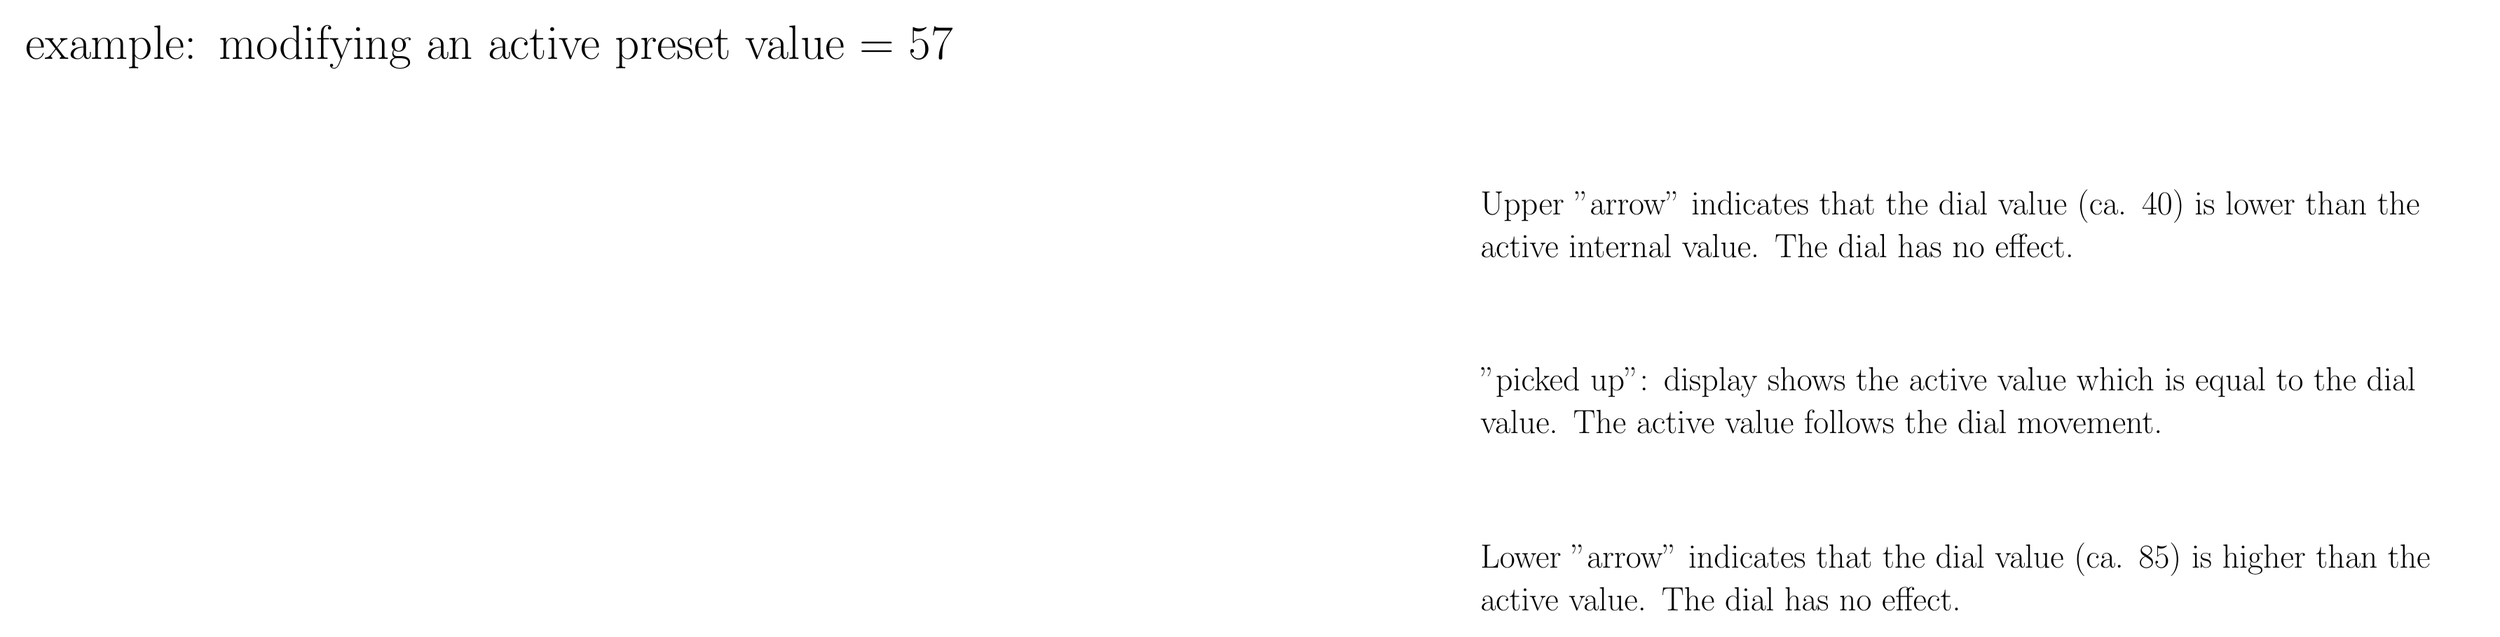
\begin{tikzpicture}[scale=0.8]
  \node[font=\fontsize{24}{22}\selectfont, align=left, outer sep=0.5mm, anchor = west, text width=40cm] at (3cm,20cm) {\presetpanel example: modifying an active preset value = 57};
    \upperbuttons{6.5cm,7.5cm}{PT}{}

    \prophetpot{26cm,8cm}{}{345}
    \prophetdisplay{32cm,8cm}{567}{}{}
    \node[font=\fontsize{18}{22}\selectfont, align=left, anchor = west, text width=18cm] at (36cm,8cm) {Lower "arrow" indicates that the dial value (ca. 85) is higher than the active value. The dial has no effect.};

    \prophetpot{26cm,12cm}{}{65}
    \prophetdisplay{32cm,12cm}{13467}{123}{}
    \node[font=\fontsize{18}{22}\selectfont, align=left, anchor = west, text width=18cm] at (36cm,12cm) {"picked up": display shows the active value which is equal to the dial value. The active value follows the dial movement.};

    \prophetpot{26cm,16cm}{}{125}
    \prophetdisplay{32cm,16cm}{}{237}{}
    \node[font=\fontsize{18}{22}\selectfont, align=left, anchor = west, text width=18cm] at (36cm,16cm) {Upper "arrow" indicates that the dial value (ca. 40) is lower than the active internal value. The dial has no effect.};
    
  \end{tikzpicture}
}

The pick-me-up mechanism avoids discontinuous value changes and it provides a means to dial the current panel into the patch you are hearing. Note, however, that it is important to observe the display and current pick-up status of dials to avoid confusion. If you want a direct application of a dial press \totape to switch back to standard \presetpatch where all control changes are directly applied. The pick-up status of each control is remembered when switching between the two modes.

There is no pick-up mechanism for switches on the panel\footnote{The attempt to do this was made, but surprisingly the hardware is not reliable enough for this. In particular, the state and intermediate states of the three-way tracking switch is somewhat random.}. The mechanism is also irrelevant for additional patch parameters as there is no conflict between physical controls and internally applied values. Furthermore, the logic applies only to patch parameters. It is not applied to \mastertune, \mastervol, \pitchbender and \modwheel.

\textbf{Default Patch}

Pressing the \preset button (with confirmation) in \shiftmode or \shiftlock loads a default patch (see section \ref{defaultpatch}). After loading the default patch the Prophet 600 is in \presetpatch.
